\section{Introduction}

Large Language Models (LLMs) now dominate natural language processing (NLP) \citep{devlin2019bert, brown2020language, kaplan2020scaling, ouyang2022training, wei2022emergent, wei2022chain, touvron2023llama, openai2024gpt4technicalreport}, powering chatbots \citep{anthropic2023claude, bai2023qwen, openai2024gpt4technicalreport, deepseekai2025deepseekr1incentivizingreasoningcapability}, search engines \citep{google2023bard, microsoft2023bing}, and programming assistants \citep{copilot, claude_3_7}. These models generate text through \textit{inference}, which imposes significant computational demands on memory and processing resources \citep{garcia2019estimation}. Systems like ChatGPT incur daily inference costs exceeding \$700,000 and contribute to substantial carbon emissions \citep{patel2023peeling, patterson2021carbon}. Efficient inference scheduling can reduce these operational costs and energy consumption \citep{strubell2019energy, desislavov2021compute} by balancing system throughput and response latency \citep{wu2022sustainable}.

Figure~\ref{fig:intro_example} illustrates how a query is processed during LLM inference. The user submits a prompt (e.g., ``Is apple a fruit?''), which then passes through two computational phases:
\begin{itemize}
    \item \emph{Prefill phase (stage 0).} Upon receiving the prompt, the model first tokenizes the input into a sequence of discrete units (e.g., ``Is'', ``apple'', ``a'', ``fruit'', ``?''). These tokens are then embedded and simultaneously processed in a single forward pass to compute the \emph{Key-Value (KV) cache}, which stores intermediate representations (i.e., attention keys and values) for each token. These precomputed values enable efficient reuse during subsequent decoding steps. This phase corresponds to Stage 0 in Figure~\ref{fig:intro_example}, where all prompt tokens are embedded and their KV representations are added to the cache.

    \item \emph{Decode phase (stages 1 to $l^\prime$).} After the prefill phase, the model enters the decode phase, where it generates the output one token at a time. At each stage, the model queries the existing KV cache to compute the next token, appends the new token to the output sequence, and updates the KV cache with its key-value pair. For instance, the model might first generate ``Yes'' (Stage 1), then ``it'' (Stage 2), followed by ``is'' (Stage 3), and finally the ``End of Sequence'' (EOS) token (Stage 4). This progression is depicted in the lower part of Figure~\ref{fig:intro_example}. Each token generation step involves both reading from and writing to the KV cache, so the KV cache grows linearly with the length of the generated sequence.
\end{itemize}

Figure~\ref{fig:intro_example} also highlights key performance metrics in LLM inference:
\begin{itemize}
    \item \emph{Time-to-first-token} (TTFT) measures the latency from user input to the first generated token.
    \item \emph{Latency} refers to the total time required to complete the generation of all output tokens.
    \item \emph{Throughput} captures the average number of tokens generated per unit time.
\end{itemize}

This inference structure, particularly the growing memory requirements and sequential decoding pattern, introduces fundamental constraints on scheduling and batching. Efficient scheduling must account for both prompt heterogeneity and KV cache dynamics to balance latency and resource use.

\begin{figure}
    \centering
    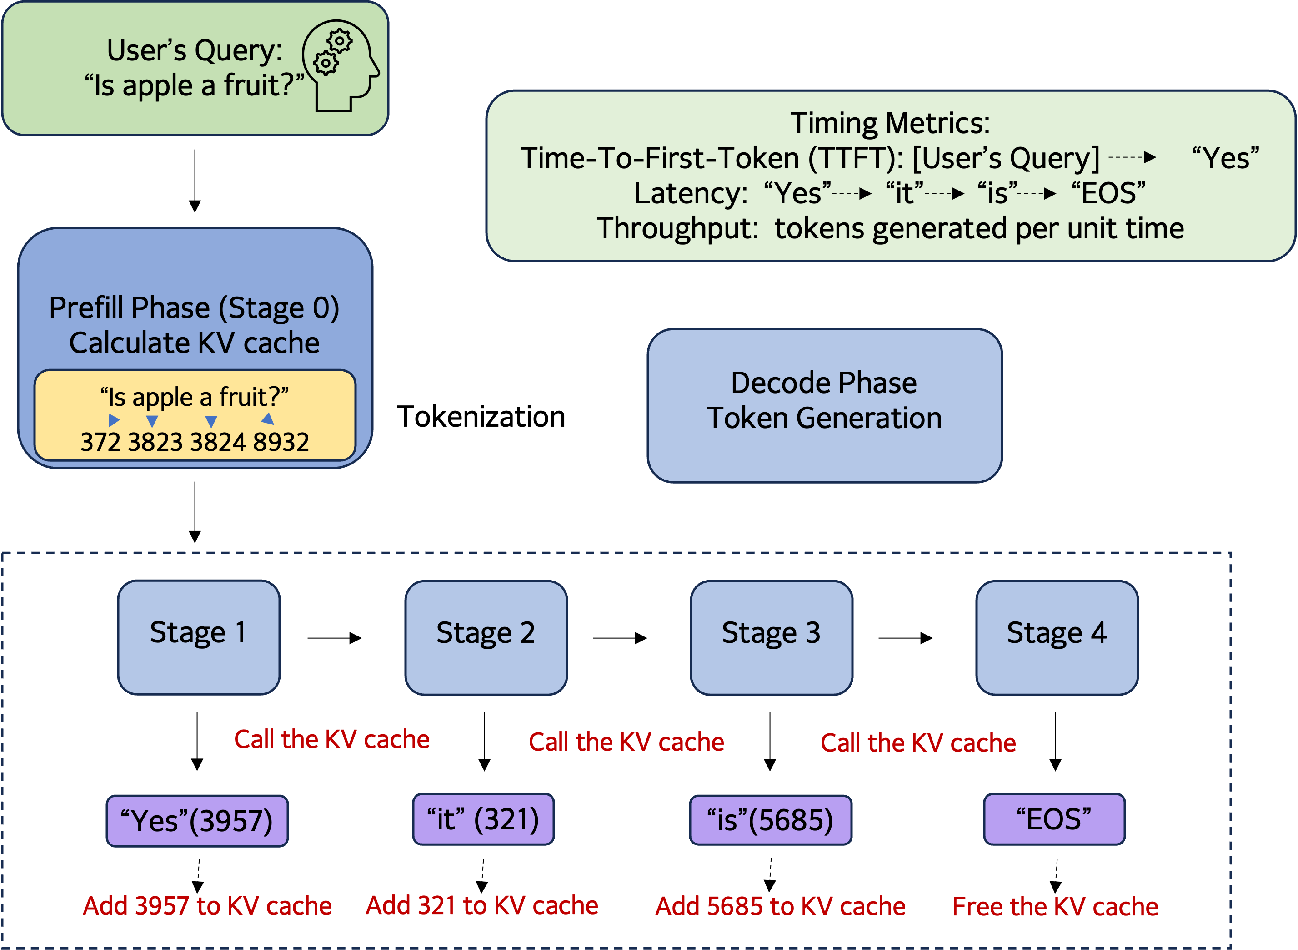
\includegraphics[width=0.55\linewidth]{Experiments_pdf/fig_intro.pdf}
    \caption{An example of LLM inference.}
    \label{fig:intro_example}
\end{figure}

Scheduling LLM inference tasks involves grouping prompts into \textit{batches} processed concurrently on a GPU. Batching improves throughput: processing multiple prompts together amortizes the fixed overhead of each iteration and better uses GPU parallelism. However, this benefit comes with a fundamental tension: larger batches consume more memory through their combined KV caches. The KV cache improves efficiency, as it prevents the model from recalculating attention history for each new token; without it, computational cost would scale quadratically with sequence length. But the KV cache also grows dynamically during decode, making memory consumption unpredictable. This creates a core trade-off: \emph{larger batches increase throughput but consume more memory, risking capacity overflow}.

Memory overflow can occur in several practical scenarios: (i) \emph{bursty arrivals}, where sudden traffic spikes temporarily exceed capacity; (ii) \emph{unknown output lengths}, where prompts generate longer responses than anticipated; and (iii) \emph{multi-tenant environments}, where multiple users compete for GPU memory. The unknown output length problem is particularly challenging: since the scheduler cannot predict how much memory each prompt will eventually consume, it cannot reliably plan batch composition or admission decisions. Traditional scheduling methods such as Shortest Job First (SJF) assume fixed job sizes and known processing times, making them unsuitable when memory demands grow unpredictably \citep{tay2022efficient, kang2024gear, hooper2025kvquant}.

When the total KV cache exceeds GPU memory capacity, the system must evict some in-progress prompts. Two approaches exist: (i) \emph{swapping} to CPU or SSD, which incurs I/O overhead \citep{sheng2023flexgen, aminabadi2022deepspeed}; and (ii) \emph{recomputation}, which discards the KV cache and restarts the prompt from prefill \citep{kwon2023efficient}. We focus on recomputation because it is the default in modern production systems such as vLLM \citep{vllm-v1-2025}, and because our goal is to \emph{minimize eviction} through scheduling rather than to optimize the eviction mechanism itself \citep{li2025mirage}. Eviction creates a vicious cycle: it frees memory temporarily, but restarted prompts consume the memory again and can trigger further evictions. Users experience this as error messages (e.g., ``Something went wrong'') or incomplete responses under heavy load.

\emph{Memory sufficiency alone does not guarantee stability.} The key to maximizing throughput is \emph{load balance}, the equilibrium state at which arrival and completion rates match. Even when total capacity $C$ exceeds the optimal steady-state memory $M^*$ (derived in our fluid analysis), naive policies can push the system away from equilibrium. For instance, first-come-first-served (FCFS) can trigger cascading evictions that reduce effective throughput, the completion rate net of evictions, by as much as $20\%$ when capacity is theoretically sufficient (Example~\ref{ex:fcfs_cascade}). A slight imbalance causes one prompt type to overflow, triggering evictions; the freed memory then fills with another type, which itself overflows, creating a vicious cycle. Thus, a system that \emph{should} be stable becomes unstable under poor scheduling.

Preventing eviction requires \emph{approaching load balance through controlled admission}. Effective scheduling demands not just sufficient capacity but keeping the system near equilibrium by controlling when prompts advance to the next decode stage. This "approaching load balance" principle guides our algorithm design: threshold-based mechanisms hold prompts at decode-stage boundaries until memory conditions permit safe continuation, keeping the system close to the fluid equilibrium. The principle yields two benefits at once. Operating near the fluid equilibrium both \emph{enlarges the stability region}, because eviction cascades no longer destabilize a system whose capacity is theoretically sufficient, and \emph{reduces mean end-to-end latency across the underloaded, near-capacity, and overloaded regimes}. In the underloaded regime, our algorithms and the baselines are all stable, yet tighter load balance still produces lower mean latency; near the stability boundary, baseline latency diverges while ours remains bounded; under sustained overload, our algorithms sustain effective throughput closer to the arrival rate. Section~\ref{sec:experiments} documents all three effects.

Recent system-level optimizations for LLM inference \citep{yu2022orca, kwon2023efficient, agrawal2023sarathi, pope2023efficiently, deepseekai2024deepseekv2strongeconomicalefficient, patel2024splitwise, zhong2024distserve} focus on engineering solutions but lack a rigorous mathematical foundation. In practice, output length predictions are imprecise or costly \citep{fu2025efficient}, and algorithms designed for known output lengths can degenerate significantly when this assumption fails (see Proposition~\ref{prop:unknown_lower_bound}).

We develop a fluid approximation that identifies the equilibrium state, at which prompt arrivals and completions balance, and characterizes the steady-state memory level $M^*$ at which the fluid system sustains the largest arrival rate. This equilibrium serves as a design target: when the stochastic system operates near it, the system sustains high effective throughput while avoiding eviction. The analysis shows that memory is a resource to exploit rather than merely a constraint, because larger batches process more prompts per iteration and increase GPU utilization.

Guided by these fluid insights, we design threshold-based algorithms that keep the stochastic system close to the fluid equilibrium. The WAIT algorithm demonstrates this for known output lengths: threshold-based admission control at each decode stage prevents the system from drifting away from balance. For unknown output lengths, we introduce Nested WAIT, which classifies prompts \emph{on the fly}: short prompts complete early and exit, while longer prompts advance to later segments, all without requiring output length prediction. Both algorithms achieve asymptotic optimality by approaching the fluid equilibrium. 

\subsection{Summary of Contributions}

Our main contributions are as follows.
\begin{itemize}
    \item \emph{Memory-constrained scheduling model.} We develop a multi-stage online scheduling model that captures the dynamic growth of KV cache memory during LLM inference, where exceeding capacity triggers costly prompt evictions (Section~\ref{sec:model}). Because the system is open, throughput equals the arrival rate whenever the policy stabilizes the system. The design goal is therefore twofold: to enlarge the stability region, and to operate near the equilibrium memory level $M^*$ required to sustain its boundary. A fluid approximation from queueing theory lets us characterize both (Section~\ref{sec:fluid}).
    \item \emph{Eviction-prevention scheduling algorithms.} We develop threshold-based algorithms that prevent memory overflow and minimize eviction. The WAIT algorithm (Section~\ref{sec:wait}) handles known output lengths; the Nested WAIT algorithm (Section~\ref{sec:nested_wait}) extends to unknown output lengths through on-the-fly type classification. A threshold at each decode-stage boundary performs a \emph{dimensionality reduction}: it decouples prompt types and replaces the continuously growing KV cache dynamics with a discrete-time per-type recursion. Both algorithms are asymptotically optimal.
    \item \emph{Experimental validation.} We evaluate our algorithms on synthetic and real-world workloads using Llama-2-7B on a single A100 GPU (Section~\ref{sec:experiments}). We compare against vLLM \citep{kwon2023efficient} and Sarathi \citep{agrawal2023sarathi}, two widely used open-source LLM inference servers that represent, respectively, memory-reactive preemptive recomputation and chunked-prefill scheduling. Consistent with the load-balancing principle, WAIT and Nested WAIT \emph{enlarge the stability region} relative to both baselines and \emph{reduce mean end-to-end latency across the underloaded, near-capacity, and overloaded regimes}; near the stability boundary, baseline latency diverges while ours remains bounded.
\end{itemize}
Our batching theory also extends naturally to Prefill-Decode Disaggregated (PD) systems such as DistServe \citep{zhong2024distserve} and Splitwise \citep{patel2024splitwise}, in which the decode server handles decode-only workloads: the linear iteration-time model in Section~\ref{sec:model} then holds exactly, the same thresholds apply, and Appendix~\ref{app:pd_disagg} reports numerical results that confirm the extension on representative PD workloads.
% The paper is structured to elucidate these advancements:
% \begin{itemize}
%     \item \textbf{Section 2} delineates the scheduling problem and its objectives.
%     \item \textbf{Section 3} details the fluid model for throughput optimization.
%     \item \textbf{Section 4} presents the booking-limit algorithm for known prompt types.
%     \item \textbf{Section 5} extends this to a nested algorithm for unknown output lengths.
%     \item \textbf{Section 6} reports numerical findings validating our approach.
%     \item \textbf{Section 7} concludes with implications and future research avenues.
% \end{itemize}

\subsection{Other Related Work}

\paragraph*{Online Scheduling Problem and Queueing System.} 
Classical online scheduling problems focus on optimally assigning jobs that arrive sequentially, each with varying completion times. In settings with stochastic arrivals, foundational studies such as \cite{devanur2009adwords,vee2010optimal,cole2014sample,balkanski2016power,lattanzi2020online} have developed algorithms that learn arrival patterns or distributions to refine scheduling strategies over time. Beyond individual job processing, works like \cite{im2013online,lucier2013efficient,liu2015online,li2020online} have explored simultaneous batching and scheduling, grouping similar jobs to enhance efficiency. Within queueing theory, fluid models serve as first-order approximations of stochastic systems, enabling near-optimal control strategies \cite{mandelbaum1998strong,maglaras2000discrete,bauerle2002optimal,liu2011network}, while asymptotic analysis characterizes long-horizon behavior. However, these traditional approaches do not account for key features of LLM inference that complicate asymptotic analysis: (i) iteration time varies with batch composition and current KV cache sizes, precluding fixed service time assumptions; (ii) memory consumption grows dynamically during decode as new tokens are generated; (iii) out-of-memory (OOM) events trigger prompt eviction, creating feedback loops that classical stability and limit theorems cannot accommodate, as those theorems assume jobs complete once started, whereas eviction invalidates standard drift arguments.

\paragraph*{LLM Inference.} 
Theoretical frameworks for analyzing Large Language Model (LLM) inference remain scarce despite the scale of production deployment. Unlike classical scheduling, LLM inference combines stochastic arrivals, dynamic memory constraints, and multi-phase prefill/decode processing. System-level works such as Splitwise \citep{patel2023peeling} and DistServe \citep{zhong2024distserve} split inference into separate prefill and decode pipelines, while scheduling engines such as Orca \citep{yu2022orca} and Sarathi \citep{agrawal2023sarathi,agrawal2024taming} improve throughput through batching and admission control. Other system-level optimizations include multi-head latent attention with low-rank KV compression \citep{deepseekai2024deepseekv2strongeconomicalefficient} and Kendall's-Tau prioritization by predicted output length \citep{fu2025efficient}. These works advance system-level efficiency through implementation and engineering. We complement them from the theoretical side, analyzing the underlying scheduling problem to characterize the stability region and the throughput gap induced by memory-growth dynamics. 
% More recently, \cite{jaillet2025onlineschedulingllminference} offers a notably theoretical framework, modeling LLM inference as an online scheduling problem and analyzing an adapted shortest-job-first algorithm with near-optimal regret—yet it assumes known output lengths at arrival, a condition rarely met in practice due to their unpredictability and estimation costs (for example, another neural network may be used at the input side). 
From an operations research perspective, several recent works analyze LLM inference scheduling under online-algorithm frameworks, focusing on competitive ratio and regret bounds. \cite{jaillet2025onlineschedulingllminference} develop an online scheduling algorithm with near-optimal regret guarantees for settings with known output lengths. \cite{wang2025llm} study optimization with variable prefill and decode lengths in pipeline-parallel settings. \cite{chen2025adaptively} address robust optimization under prediction uncertainty, considering adversarial scenarios. A different theoretical angle is taken by \cite{li2025throughput}, whose stochastic processing model allows general batch processing times, including a piecewise-linear form that captures the compute-bound / memory-bound transition, and shows that work-conserving algorithms achieve the fluid-optimal throughput. On output length uncertainty, \cite{jaillet2025onlineschedulingllminference} and \cite{wang2025llm} assume lengths are known at arrival, \cite{chen2025adaptively} considers adversarial unknown lengths, while our Nested WAIT algorithm handles stochastic unknown lengths through on-the-fly classification at segment boundaries. These works establish competitive-ratio or regret guarantees relative to hindsight benchmarks. Our work takes a different angle: a fluid-based analysis that characterizes the stability region through a memory-dependent iteration-time model (Equation~\eqref{eq:time_consump}), showing that threshold-based admission \emph{enlarges} this region by preventing eviction cascades.


\subsection{Notations}
For integer $n\ge 1,$ we denote $[n]=\{1,2,\dots,n\}$ as the set of integers from $1$ to $n$. For $x\in\real$, denote $\lceil x\rceil$ as the smallest integer not smaller than $x$ and $\lfloor x\rfloor$ as the largest integer not greater than $x$. Denote $x_+=\max\{x, 0\}$. For set $S$, denote $|S|$ as its cardinality. For two functions $f(T)$ and $g(T)$, we use $f(T)=O(g(T))$ if there exists constant $c_1>0$ such that $f(T)\le c_1g(T)$ as $T\to+\infty$ and $f(T)=\Omega(g(T))$ if there exists constant $c_2>0$ such that $f(T)\ge c_2g(T)$ as $T\to +\infty$. 
